%----------------------------------------------------------------
%
%  File    :  chapter3.tex
%
%  Authors : Michael Fuska, FH Campus Wien, Austria
% 
%  Created : 13 Feb 2016
%
%  Changed :  
% 
%----------------------------------------------------------------


\chapter{Jailbreak}
\label{ch:JB}

% ------------- JB Allgemein --------------------
\section{Allgemein}
\label{sec:JBAllgemein}

Mit Hilfe eines \textbf{Jailbreaks} kann der User Apps installieren die nicht von Apple signiert und verteilt worden sind. Um dies zu ermöglichen muss ein Jailbreak die Sicherheitsmechanismen von Apple umgehen. Weiters erhält der User den Zugriff auf den \textit{\glqq Root-Users\grqq{}} des Devices. Der \textit{\glqq Root-User Loggin\grqq{}} ermöglicht vollen Zugriff auf das Betriebssystem (iOS) und somit auf alle Daten des Devices. Durch die Installation eines Jailbreaks stehen zwei weitere \textit{\glqq App Stores\grqq{}} zur Verfügung

\begin{description}
\item[Alle von Apple nicht autorisierten App Stores]~
	\begin{enumerate}
	   	\item \textbf{Cydia} \cite{Cydia[1]}
		\item \textbf{TaiG}
	\end{enumerate}
\end{description}

% ------------- Arten JB --------------------
\section{Arten von Jailbreaks}
\label{sec:JBArten}
Abhängig davon wie sich ein iOS Device nach dem Reboot des Devices verhält, unterscheidet man zwischen drei Arten von Jailbreaks. 

% ------------- Tethered Jailbreak--------------------
\subsection{Tethered Jailbreak}
\label{sec:JBTethered}
Nach der Installation eines \textbf{Tethered-Jailbreaks} ist es nicht möglich das Device ohne weitere Tool neu zu starten. Nach einem Neustart des iOS, startet das Betriebssystem in dem sogenannten \textit{\glqq DFU Mode\grqq{}}. \par
Mit dem zuvor an PC installierten Jailbreak Tool kann das Device wieder gestartet werden. Es wird in den selben Zustand versetzt, wie vor dem Reboot. Nur mit Hilfe von iTunes kann auf dem Device wieder die originale iOS Software installiert werden. 
\begin{description}
     \item[\parbox{\textwidth} {Nachfolgend werden zwei häufig verwendet Tethered-Jailbreak Tools angeführt}]~\par
    \item[]~\par
	\begin{itemize}
            \item \textbf{redsn0w}
            \item \textbf{Blackra1n}
    \end{itemize}
\end{description} 

% ------------- Semi Tethered Jailbreak--------------------
\subsection{Semi Tethered Jailbreak}
\label{sec:JBSemiTethered}

Nach der Installation eines \textbf{Semi-Tethered Jailbreak} kann das iOS Device neugestartet werden. Das System startet nicht in den DFU Mode, sondern in einen eingeschränkt funktionsfähigen Betreibsmodus. Safari, Mail, Cydia und alle Apps die mit iTunes installiert worden sind, können nach einem Neustart weiterhin verwendet werden. Bei der Installation des Jailbreaks wird auch eine App am Device installiert, diese muss nach einem Neustart ausgeführt werden um das Device wieder in den selben Zustand zu versetzen, wie vor dem Reboot. Danach ist das iOS Device wieder vollständig funktionsfähig.

\begin{description}
    \item[Ein Beispiel für einen Semi-Tethered Jailbreak ist]~\par
	\begin{itemize}
        \item \textbf{SemiTether (Cydia package)}
    \end{itemize}
\end{description} 

% ------------- UnTethered Jailbreak--------------------
\subsection{Untethered Jailbreak}
\label{sec:JBUntethered}
Wurde auf dem iOS Device ein \textbf{Untethered Jailbreak} installiert, ist das iOS Device nach dem Neustart des Systems wieder voll funktionsfähig.
\begin{description}
\item[\parbox{\textwidth} {Einige Beispiele für Untethered Jailbreaks sind}]~\par
	\begin{multicols}{2}
	\begin{itemize}
        \item \textbf{Absinthe}
        \item \textbf{evasi0n7}
        \item \textbf{Pangu}
        \item \textbf{Pangu8}
        \item \textbf{Pangu9}
        \item \textbf{TaiG}
    \end{itemize}
    \end{multicols}
\end{description} 

% ------------- Semi Untethered Jailbreak--------------------
% \subsection{Semi Untethered Jailbreak}
% \label{sec:JBSemiUntethered}

% ------------- Jailbreak History --------------------
\section{Jailbreak History}
\label{sec:JBHistory}
Apple veröffentlicht im Durchschnitt sieben iOS Updates pro Jahr.

\begin{description}
\item[\parbox{\textwidth} {Die Software-Updates dienen dazu}]~\par
	\begin{enumerate}
	    \item Die Sicherheitslücken des Betriebssystems zu schließen
	    \item Neue Sicherheitsmechanismen für das Betriebssystem und Apps einzuführen
	    \item Neue Sicherheitsarchitekturen für Apps bereitzustellen
	\end{enumerate}
\end{description} 
 
Seit der Veröffentlichung der ersten iOS Version im Jahr 2007 wurden insgesamt 79 Softwareupdates von Apple bereitgestellt. Darunter befinden sich neun Major-Updates und 70  Minor-Updates. Siehe Figure \ref{fig:iOS Software Updates}.

\begin{figure}[!ht]
        \centering
                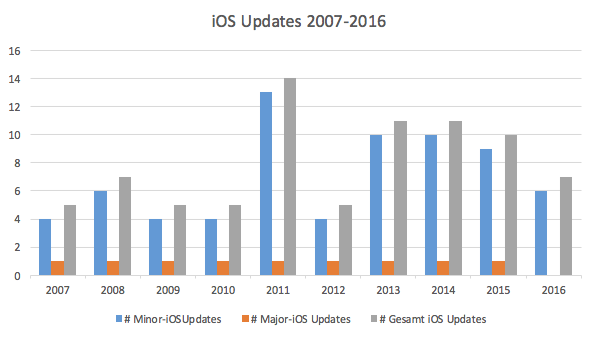
\includegraphics[scale=0.7]{Bilder/iOSUpdates1}
        \caption{iOS Software Updates\cite{Apple[7]}}
        	\label{fig:iOS Software Updates}
\end{figure}

Die Jailbreak-Community benötigt im Durchschnitt 36 Tage, um die Sicherheitsmechanismen von Apple zu umgehen. Die iOS Bugs, die für ein Jailbreak verwendet werden sind meistens in mehreren iOS Versionen vorhanden. Nicht alle Software Fehler werden von Apple geschlossen, es gibt Jailbreaks, die mehrere Jahre funktionieren. Dies gilt vor allem für ältere iOS Versionen und iOS Devices. Im Durchschnitt werden pro Jahr zwei Jailbreak veröffentlicht. Siehe Abbildung \ref{fig:iOS Jailbreak}.

\begin{figure}[!ht]
        \centering
                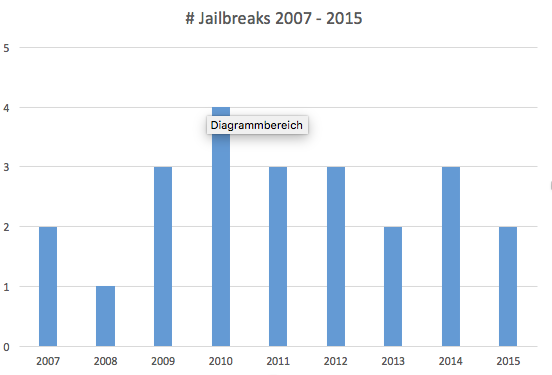
\includegraphics[scale=0.7]{Bilder/AnzahlJB}
        \caption{Anzahl iOS Jailbreak 2007 - 2015}
        	\label{fig:iOS Jailbreak}
\end{figure}


% ------------- Aufbau Jailbreak 9.x --------------------
\section{Aufbau Jailbreak iOS 9.x}
\label{sec:JBAufbau}
Um ein Jailbreak auf einem iOS Device erfolgreich durchführen zu können, muss Schritt für Schritt jeder Sicherheitsmechanismus des iOS ausgehebelt werden. Ab der iOS Version 8.1.3 müssen folgende Sicherheitsvorkehrungen umgangen werden um einen untethered Jailbreak durchzuführen.

\begin{enumerate}
	    \item \textbf{Secure Boot Chain} (siehe Kapitel: \ref{sec:SecBootChain})
	    \item \textbf{ALSR }(siehe Kapitel: \ref{sec:ASLR}) 
	    \item \textbf{Code Signing}(siehe Kapitel: \ref{sec:SigningProcess}) 	   
	    \item \textbf{Sandbox} (siehe Kapitel: \ref{sec:Sandbox}) 
\end{enumerate}

\begin{description}
    \item[\parbox{\textwidth} {Damit die Sicherheitsmechanismen überhaupt umgangen werden können, müssen verschiedene Programmierfehler im iOS gefunden werden. }]~\par
  \begin{enumerate}
  \item \textbf{Einen oder mehrere Softwarefehler, die das Umgehen der iOS Sicherheitsmechanismen ermöglichen.}
  \item \textbf{Einen oder mehrere Softwarefehler, die es dem Jailbreak ermöglichen Root-Rechte zu erhalten.}
  \item \textbf{Einen oder mehrere Softwarefehler, die das Patchen des Kernels ermöglichen. Das Patchen des Kernels ist nur notwendig, wenn ein untethered Jailbreak durchgeführt werden soll}
\end{enumerate}\end{description} 
(Vgl. \cite{TaiG[1], TaiG[2], TaiG[3]})

Andreas Kurtz definiert dies in seinem Fachartikel wie folgt: \textit{\glqq Die meisten Verfahren gründen auf zwei oder mehr Software-Schwachstellen: Einer Schwachstelle in einer der Userland-Komponenten, also etwa einer App, und mindestens einer weiteren, die sich zur Rechteerweiterung nutzen lässt. Mittels der ersten wird zunächst Code im Kontext der Userland- Komponente ausgeführt, beispielsweise im Webbrowser. Von dort ausgehend werden weitere Schwachstellen ausgenutzt, um die Rechte zu erweitern und um Sicherheitsmechanismen zu deaktivieren.\grqq{}} \cite{JB[2]}

% ------------- Jailbreak Step 1 --------------------
%\subsection{Breaking out of the sandbox}
%\label{sec:JBStep1}
%Im ersten Schritt muss ein Bug im iOS und/oder einer Applikation gefunden werden, welcher es erlaubt \glqq die Sandbox\grqq{} (siehe Kapitel: \ref{sec:Sandbox}) zu umgehen. 

% ------------- Jailbreak Step 2 --------------------
%\subsection{Obtaining arbitrary (unsigned) code execution}
%\label{sec:JBStep2}

% ------------- Jailbreak Step 3 --------------------
%\subsection{Obtaining root}
%\label{sec:JBStep3}

% ------------- Jailbreak Step 4 --------------------
%\subsection{Patching the Kernel}
%\label{sec:JBStep4}

%AFC -> /private/var/mobile/Media Verzeichnis un dem jeder Prozess lesen und schreiben darf Einstiegspunkt
%/private/var/mobile/ ist homeverzeichnis für nicht root user
%/private/var/run/mobile_image_mounter -> ../../../var/mobile/Media/Books/Purchases/mload 


%AFC \glqq Apple File Conduit \grqq{} ist ein Service welches es ermöglicht Files und Verzeichnisse mit dem Device über USB auszutauschen bzw erstellen. AFC wird von iTunes verwendet. 
%DDI ist ein Teil der SDK und enthält Tools und Framework. Weiters wurde das  DDI von Apple signiert und ist somit vor Veränderungen geschützt. 

%Ersetzen des Development Disk Image (DDI) damit die  folgende Dateien ersetzt werden können. "/usr/lib/libmis.dylib" und "/usr/lib/xpcd_cache.dylib"


